\chapter{TrueSkill\texttrademark~Rating System}\label{Chap:3}
TrueSkill~\cite{TS07} is a Gaussian rating system developed by Microsoft Research in 2007 to rank players on Xbox Live for the purpose of creating competitive matches amongst players with similar skill levels. While the Elo rating system is applicable to only two-player matches, the TrueSkill ranking system extends the use cases to multi-player matches. Section~\ref{Sec: tmm} describes Approximate Bayesian Inference --- the mathematical backbone of the TrueSkill rating system and Section~\ref{Sec: imp} discusses the prediction performances of several models built upon an open-source implementation of the TrueSkill rating system. 

\section{Approximate Bayesian Inference}\label{Sec: tmm}

The approach described in Section~\ref{Sec: approach} can be modelled as a Bayesian Inference process. Define a vector $\matr{s}  = [s_{1}, s_{2}, \ldots, s_{n}]^{\intercal}$ representing the individual \emph{skill} of $n$ teams in a match (in the case of NCAA basketball tournament, $n = 2$). Further assume that each skill follows a Gaussian distribution $s_{i} \sim \mathcal{N}(\mu_{i}, \sigma_{i}^{2})$ and collectively, the \emph{prior} joint distribution of skills is a n-variate Gaussian distribution $p(\matr{s}) = \mathcal{N}_{n}(\matr{s}; \matr{\mu}, \matr{\Sigma})$.

In a match, each team is expected to exhibit a certain \emph{performance} $p_{i} \sim \mathcal{N}(s_{i}, \beta_{i}^{2})$ that varies around its skill. The match result can be represented as a set of rankings in ascending order for each team, namely, $\matr{r} = [r_{1}, r_{2}, \ldots, r_{n}]^{\intercal}$ where $r_{1} \leq r_{2}, \ldots, r_{n - 1} \leq r_{n}$. In reality, there are many factors that may affect the outcome of a match, but for the purpose of Bayesian Inference, the assumption is that it is the differences in team performances that cause the differences in team rankings. According to the Bayes' Theorem, the posterior distribution $p(\matr{s} | \matr{r})$ is given by
\begin{equation}\label{Eqn: bayes}
p(\matr{s} | \matr{r}) = \frac{P(\matr{r} | \matr{s})p(\matr{s})}{P(\matr{r})} = \frac{P(\matr{r} | \matr{s})p(\matr{s})}{\int P(\matr{r} | \matr{s})p(\matr{s})d\matr{s}}
\end{equation}

The above formula demonstrates the use of Bayes' Theorem to calculate the updated skill distribution (posterior) given the match outcome (evidence) and the expectations (likelihood and prior) on the match outcome before the match. However, the posterior distribution is no longer a Gaussian distribution and oftentimes, the integral is intractable. A common solution is to calculate a Gaussian distribution $\mathcal{N}_{n}(\matr{s}; \hat{\matr{\mu}}, \hat{\matr{\Sigma}})$ as an approximation to the posterior distribution $p(\matr{s} | \matr{r})$ so that the Kullback-Leibler divergence between the two distributions is minimised. 

A number of approximation techniques are available. For the TrueSkill rating system, it approximates the posterior distribution by setting up a \emph{factor graph} which is a bipartite graph containing two kinds of vertices: variables and factors. A variable stores some value of interests and a factor represents some operations on one or more variables. The Bayesian Inference process is modelled as passing some \emph{message}s, which are some real-valued functions of a variable or a factor, throughout the factor graph. Figure~\ref{Fig:fact_grph} shows an example factor graph of a simple two-player match. Based on skill $s_{i}$ and performance $p_{i}$, it calculates the expected performance difference $p_{1} - p_{2}$ and compares that with an externally supplied outcome $d$. The $\mathbb{I}$ denotes an indicator function to assert whether $d$ is consistent with the expectation, depending on which a different update is performed on $s_{1}$ and $s_{2}$. 

\begin{figure}[h!]
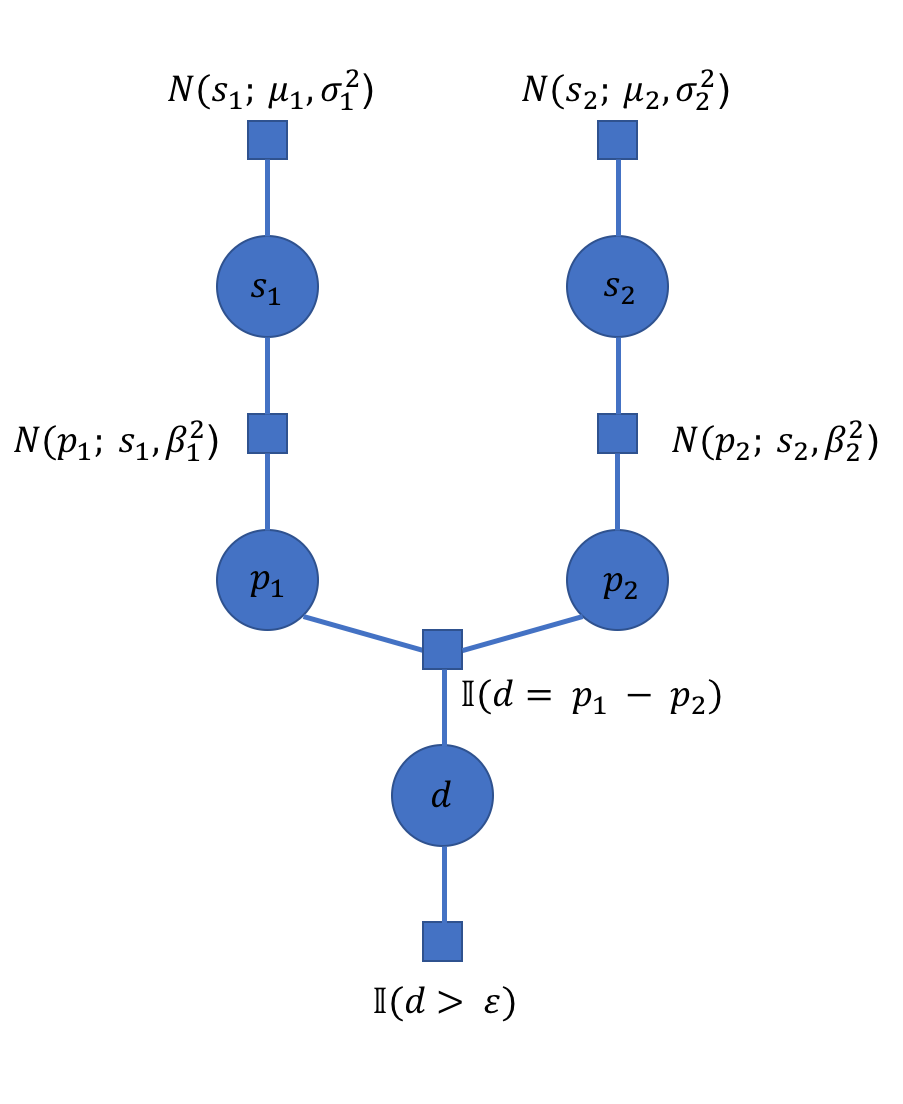
\includegraphics[scale=0.5]{factor_graph}
\centering
\caption{An example of factor graph}\label{Fig:fact_grph}
\end{figure}

The ultimate goal of a factor graph is to obtain a set of update equations that indicate how each $\mu_{i}$ and $\sigma_{i}$ should be updated. However, passing messages throughout larger factor graphs can involve very intensive computations. As suggested by~\cite{RC11}, there is an alternative but easier way of getting the same set of update equations based the following theorem. 
\begin{theorem}\label{Thrm: th1}
Let $\matr{z}$ be a k-dimensional random vector $[z_{1}, z_{2}, \ldots, z_{k}]^{\intercal}$ with a probability distribution function of the form
\begin{equation}\label{Eqn: z_dist}
\frac{\phi_{k}(\matr{z})f(\matr{z})}{\int \phi_{k}(\matr{z})f(\matr{z})d\matr{z}}
\end{equation}
where $\phi_{k}$ is a k-variate standard Gaussian distribution function. Then, the expectation of $\matr{z}$ is given by
\begin{equation}
E[\matr{z}] = E\Big{[}\frac{\nabla f(\matr{z})}{f(\matr{z})}\Big{]}
\end{equation}
and also
\begin{equation}
E[z_{i}z_{j}] = \delta_{ij} + E\Big{[}\frac{\nabla^{2} f(\matr{z})}{f(\matr{z})}\Big{]}
\end{equation}
where $\delta_{ij} = 1$ if $i = j$ and $\delta_{ij} = 0$ otherwise. 
\end{theorem}

To link Equation~\ref{Eqn: z_dist} with the Bayes' Theorem in Equation~\ref{Eqn: bayes}, notice that the match outcome is dependent on performances and performances are related to skills; therefore, the likelihood probability $P(\matr{r} | \matr{s})$ can be expressed as some function of skill $f : \matr{s} \rightarrow [0, 1]$. Furthermore, since each $s_{i} \sim \mathcal{N}(\mu_{i}, \sigma_{i}^{2})$, define the z-score vector $\matr{z} = [z_{1}, z_{2}, \ldots, z_{n}]^{\intercal}$ where 
\begin{equation}
z_{i} = \frac{s_{i} - \mu_{i}}{\sigma_{i}} 
\end{equation}
Therefore, the probability distribution $p(\matr{z}) = \phi_{n}(\matr{z})$ and the likelihood probability $P(\matr{r} | \matr{s})$ is also a function of $\matr{z}$. Then according to Equation~\ref{Eqn: bayes}, 
\begin{equation}
p(\matr{z} | \matr{r}) = \frac{P(\matr{r} | \matr{z})p(\matr{z})}{P(\matr{r})} = \frac{\phi_{n}(\matr{z})f(\matr{z})}{\int \phi_{n}(\matr{z})f(\matr{z})d\matr{z}}
\end{equation}
and therefore by Theorem~\ref{Thrm: th1}, the values of interest $\mu_{i}^{new}$ and $\sigma_{i}^{new}$ are related to $E[z_{i}]$ through

\begin{equation}\label{Eqn: mu_update}
\begin{split}
\mu_{i}^{new} &= E[s_{i}] = E[\mu_{i} + \sigma_{i}z_{i}] = \mu_{i} + \sigma_{i}E[z_{i}] \\ 
&= \mu_{i} + \sigma_{i}E\Big{[}\frac{\partial f(\matr{z}) / \partial z_{i}}{f(\matr{z})}\Big{]}
\end{split}
\end{equation}
and
\begin{equation}\label{Eqn: sigma_update}
\begin{split}
\sigma_{i}^{new} &= Var[s_{i}] = \sigma_{i}^{2}Var[z_{i}] = \sigma_{i}^{2}(E[z_{i}^{2}] - E[z_{i}]^{2}) \\
&= \sigma_{i}^{2}\Big{(}1 + E\Big{[}\frac{\nabla^{2} f(\matr{z})}{f(\matr{z})}\Big{]}_{ii} - E\Big{[}\frac{\partial f(\matr{z}) / \partial z_{i}}{f(\matr{z})}\Big{]}^{2}\Big{)}
\end{split}
\end{equation}

The above update equations are applicable to the general cases where $n$ teams are involved. However, for NCAA tournament matches that are between only two teams, a simpler version of the update equation can be derived. Now consider two teams with skill $\matr{s} = [s_{i}, s_{j}]^{\intercal}$. In general, there is no draw in basketball matches, but for completeness, assume the \emph{draw margin} is $\varepsilon$ such that team $i$ beats team $j$ when $s_{i} - s_{j} > \varepsilon$ and the outcome is considered as draw when $| s_{i} - s_{j} | \leq \varepsilon$. Furthermore, define $c^{2} = 2\beta^{2} + \sigma_{i}^{2} + \sigma_{j}^{2}$. Then 
\begin{equation}
f(\matr{z}) = \Phi \Big{(} \frac{\mu_{i} - \mu_{j} - \varepsilon}{c}  \Big{)}
\end{equation}
when team $i$ beats team $j$. Alternatively, 
\begin{equation}
f(\matr{z}) = \Phi \Big{(} \frac{\varepsilon - (\mu_{i} - \mu_{j}) }{c}  \Big{)} - \Phi \Big{(} \frac{- \varepsilon - (\mu_{i} - \mu_{j}) }{c}  \Big{)}
\end{equation}
when team $i$ draws with team$j$. In both cases, $\Phi$ represents the standard Gaussian cumulative distribution function. 

Another approximation applied above is to assume $\matr{z} = \matr{0}$, namely, the two teams are assumed to have skills that are equal to their mean skills ($\matr{s} = \matr{\mu}$). The rationale for the above equations is to construct a Gaussian difference distribution~\cite{WR17} $\mathcal{N}_{i - j}(s_{i - j}; \mu_{i} - \mu_{j}, c^{2})$ considering the performance variance $\beta^{2}$. Then for the case that team $i$ beats team $j$, it is to calculate the probability that $\mu_{i} - \mu_{j} - \varepsilon > 0$ using a standard Gaussian $\Phi$ function. Similar arguments apply to the draw case. 

Now that $f(\matr{z})$ is known, for the case team $i$ beats team $j$
\begin{equation}
\begin{split}
\frac{\partial f(\matr{z})}{\partial z_{i}} &= \frac{\partial f(\matr{z})}{\partial \mu_{i}} \cdot \frac{\partial \mu_{i}}{\partial z_{i}} = \sigma_{i}\frac{\partial}{\partial \mu_{i}}\Phi \Big{(} \frac{\mu_{i} - \mu_{j} - \varepsilon}{c}  \Big{)} \\
&= \frac{\sigma_{i}}{c} \phi \Big{(} \frac{\mu_{i} - \mu_{j} - \varepsilon}{c}  \Big{)}
\end{split}
\end{equation}
where $\phi$ is the standard Gaussian probability density function. Following Equation~\ref{Eqn: mu_update} and~\ref{Eqn: sigma_update} , the skill of team $i$ can be updated accordingly:
\begin{equation}
\mu_{i}^{new} = \mu_{i} + \frac{\sigma_{i}^{2}}{c} \cdot \frac{\phi \Big{(} \frac{\mu_{i} - \mu_{j} - \varepsilon}{c}  \Big{)}}{\Phi \Big{(} \frac{\mu_{i} - \mu_{j} - \varepsilon}{c}  \Big{)}}
\end{equation}
\begin{equation}
\sigma_{i}^{new} = \sigma_{i}^{2} 
\Bigg{\{} 
1 + \frac{\sigma_{i}^{2}}{c} 
\Bigg{[} 
-\frac{\mu_{i} - \mu_{j} - \varepsilon}{c^{2}} \cdot \frac{\phi \Big{(} \frac{\mu_{i} - \mu_{j} - \varepsilon}{c}  \Big{)}}{\Phi \Big{(} \frac{\mu_{i} - \mu_{j} - \varepsilon}{c}  \Big{)}}
-\frac{1}{c} \cdot  \frac{\phi \Big{(} \frac{\mu_{i} - \mu_{j} - \varepsilon}{c}  \Big{)}^{2}}{\Phi \Big{(} \frac{\mu_{i} - \mu_{j} - \varepsilon}{c}
 \Big{)}^{2}}
\Bigg{]}
\Bigg{\}}
\end{equation}

Detailed derivations are omitted and can be found in~\cite{RC11}. Update equations for team $j$ and for the case of draw can be derived in a similar way. By means of Approximate Bayesian Inference, the TrueSkill rating system is able to update the skill of each team upon the end of a match and to estimate a team's probability of winning an upcoming match. 

\section{Kaggle Results \& Discussions}\label{Sec: imp}

Section~\ref{SSec: features} lists many potential features that can be used as inputs to a predictive model. However, the required inputs to a TrueSkill rating system are very simple --- the winning and losing team for a particular match. It does not even take into consideration by how many points the winning team leads the losing team, which is also known as margin of victory (MOV). 

But some other features may provide valuable insights into the ``true skill'' of a team. For example, the feature `Wloc', whether the winning team was at its home court, a neutral site or the losing team's court, indicates whether the winning team was granted the ``Home Court Advantage (HCA)''. HCA can sometimes improve a team's \emph{performance} significantly and lead to a victory even if the ``true skill'' of that team is lower than its opponent's. 

Since TrueSkill does not accept these features as inputs directly, to incorporate them into the predictive models, their magnitudes are converted into some effects on the MOV of a match. For instance, HCA may be worth five points in a basketball game and therefore, five points are deducted from the winning team's final score, which may possibly result in a \emph{reverse} of the match outcome. Adjustments of this kind are carried out before the match records are fed to TrueSkill. The final features used in this project are summarised in Table~\ref{Ta:sele_feature}. 

\begin{table}[h!]
\centering
\begin{tabular}{ | l | l | }
\hline
\textbf{Feature} & \textbf{Possible Effects} \\ \hline
Wteam & Identifies the winning team \\ \hline
Wscore & Identifies the winning team's score \\ \hline
Lteam &  Identifies the losing team \\ \hline
Lscore & Identifies the losing team's score \\ \hline
MOV & The larger the MOV, the larger the skill gap \\\hline 
Wloc & Identifies whether HCA exists \\ \hline
Numot & The more overtimes, the smaller the skill gap \\ \hline
Wto & The less turnovers, the stronger the skill \\ \hline
\end{tabular}
\caption{A Summary of the Selected Features and Effectives}\label{Ta:sele_feature}
\end{table}

A larger MOV may be a good indicator of a larger skill gap between the winning team and the losing team. In this project, the effect of MOV is added iteratively: as long as the MOV is larger than some threshold value $m$, the match is considered a victory for the winning team and fed to TrueSkill, after which the MOV is deducted by $m$ and the process continues until MOV $<m$. Therefore, it is possible that an actual match is treated as \emph{multiple} victories because the match has a very large MOV. Although TrueSkill does not consider MOV, the \emph{number} of victories does matter in TrueSkill. 

Occasionally, there is overtime in a basketball match if two teams tie at the end of the normal hours. According to the rules of basketball, additional overtime must be given if two teams still tie after the last overtime. In the case of multiple overtime, it is true that there will be a winner eventually, but the fact that the first overtime happens already provides some important information about the two teams' skill levels --- they should have close skill levels that cause overtime. In this project, whenever overtime occurs in a match, regardless of how many times it occurs, the scores of the two teams are made equal to reflect this intuition. 

Turnovers can be thought as mistakes a team made in a match. There are many possible factors from both the team and its opponents that can cause turnovers, such as a double dribble or the ball being stolen. Therefore, it is a very comprehensive feature that may contain information from many other invisible factors. In this project, if a team commits more turnovers than its opponents', then its final score will be deducted by some variable amounts. 

Table~\ref{Ta:results} summaries all the models built in this project and their respective ranks on Kaggle's leaderboard. 

\begin{table}[h!]
\centering
\begin{tabular}{ | l | l | l | l | l |}
\hline
\textbf{Model No.} & \textbf{Feature Used} & \textbf{LogLoss} & \textbf{Rank} & \textbf{Top} \\ \hline
1 & Na\"{i}ve TrueSkill & 0.531040 & \nth{13} & 2.17\% \\ \hline
2 & MOV & 0.538214 & \nth{34} & 5.68\% \\ \hline
3 & HCA & 0.513445 & \nth{5} & 0.83\%\\ \hline
4 & Overtime & 0.514140 & \nth{5} & 0.83\% \\ \hline
5 & Turnover  & 0.503654 & \nth{3} & 0.50\%\\ \hline
\end{tabular}
\caption{A summary of the final results}\label{Ta:results}
\end{table}

\begin{table}[h!]
\centering
\begin{tabular}{ | l | l | l | l | l |}
\hline
\textbf{Model No.} & \textbf{Feature Used} & \textbf{LogLoss} & \textbf{Rank} & \textbf{Top} \\ \hline
1 & Na\"{i}ve TrueSkill & 1.542861 & \nth{585} & 97.66\% \\ \hline
2 & MOV & 2.046105 & \nth{593} & 99.00\% \\ \hline
3 & HCA & 0.505484 & \nth{3} & 0.50\%\\ \hline
4 & Overtime & 0.504135 & \nth{3} & 0.50\% \\ \hline
5 & Turnover  & 0.493128 & \nth{2} & 0.33\%\\ \hline
\end{tabular}
\caption{A summary of the final results}\label{Ta:results_ft}
\end{table}